% ============================================================
%  abstract_ar.tex — Arabic abstract
% ============================================================
% This includes a single pre-rendered PDF page (frontmatter/abstract_ar.pdf),
% which already has correct right-to-left layout, Arabic typeface, and the
% keywords line, exported from the reviewed Word version of this thesis.
%
% Why this approach instead of typing the Arabic directly in this .tex file:
% native Arabic via polyglossia+bidi imposes a strict load-order on every
% other package in the preamble, which is a poor trade for one page on a
% first LaTeX project. See the note in preamble.tex if you want to switch
% to native text later (e.g. because you need to revise the Arabic wording
% after the English text changes -- in that case regenerate the PDF page
% from Word/LibreOffice with RTL set, and overwrite abstract_ar.pdf; no
% change to this file is needed).

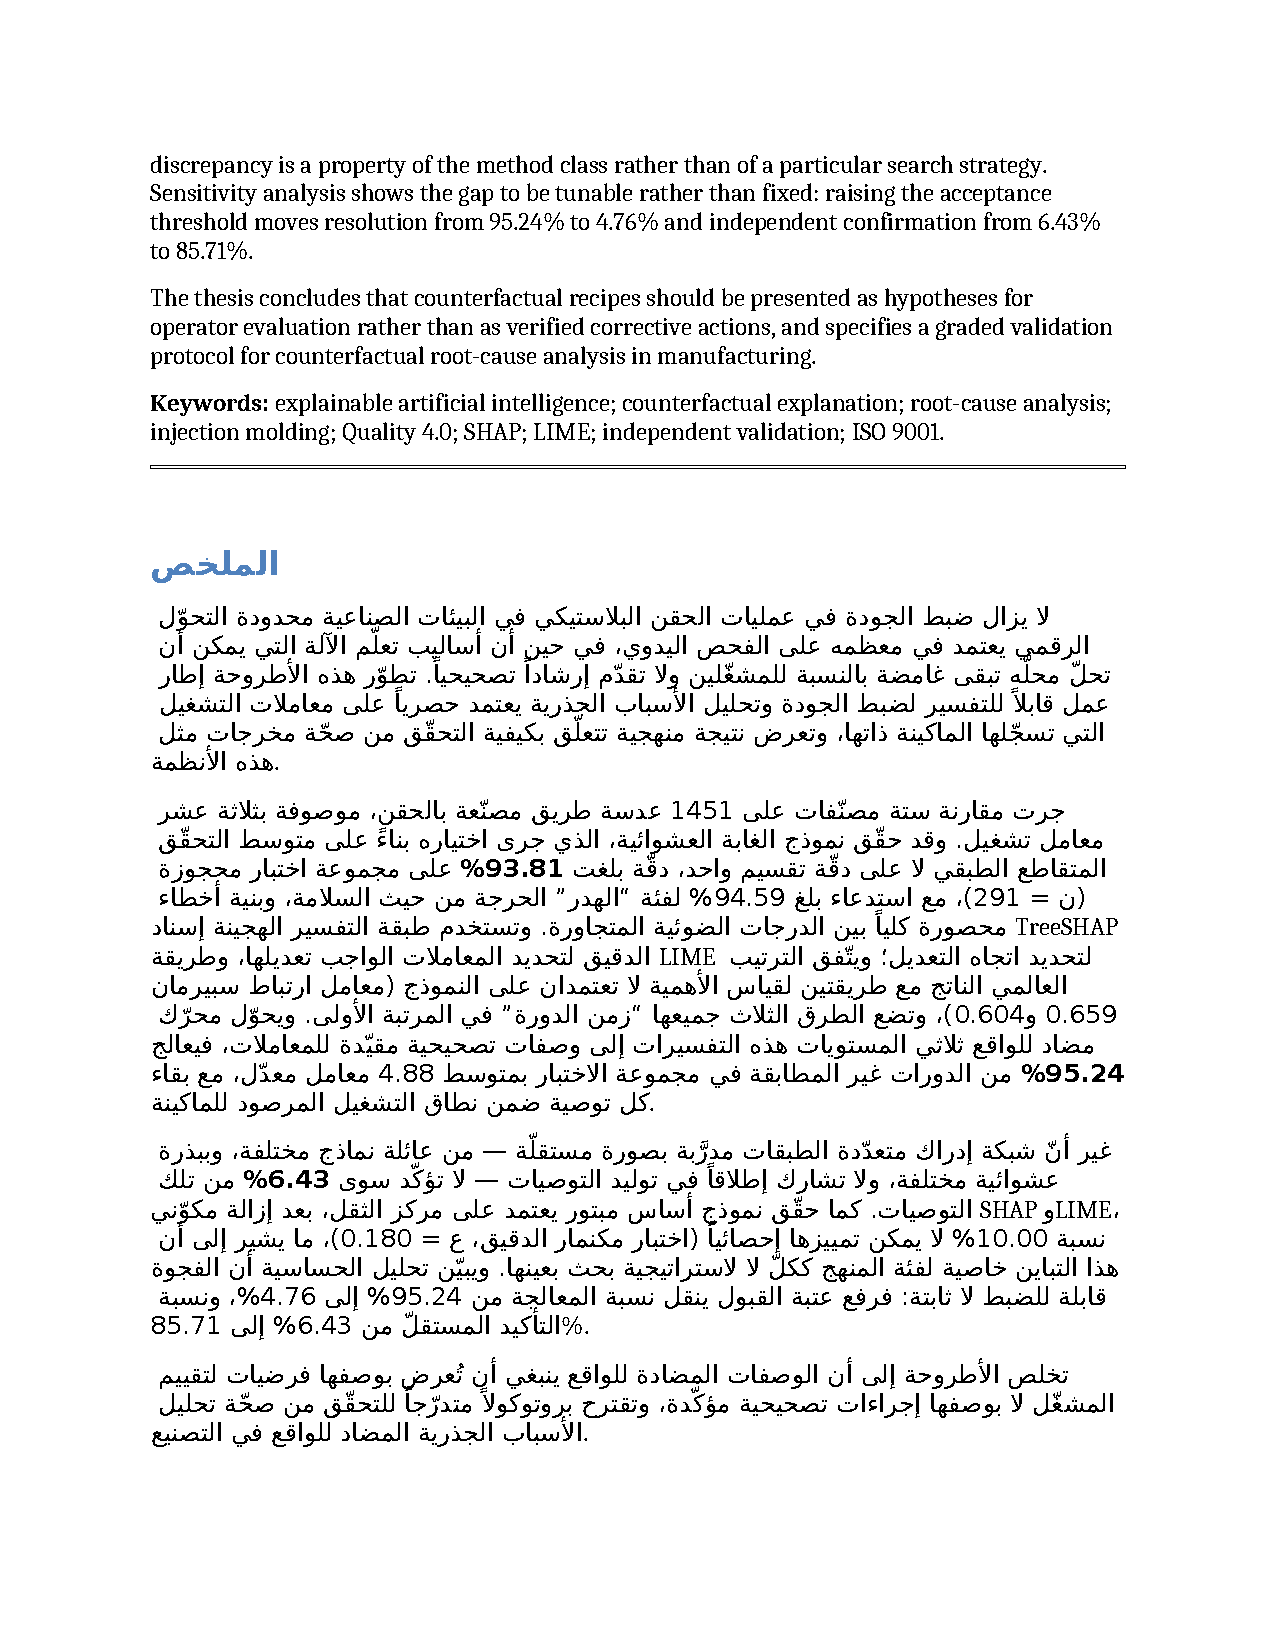
\includepdf[pages=-,pagecommand={
  \thispagestyle{empty}
  \addcontentsline{toc}{chapter}{Arabic Abstract}
}]{frontmatter/abstract_ar.pdf}
